%! Author = adnansiddiquei
%! Date = 04/06/2024

\section{Results}\label{sec:results}
To assess the performance of our reproduction, we compare the results of our implementation with the original AstroCLIP
results on the downstream tasks of redshift prediction and retrieval by cosine similarity.

\subsection{Zero-Shot k-NN Redshift Regression}\label{subsec:results-redshift-regression}
\begin{figure}[htb]
    \centering
    \makebox[\textwidth]{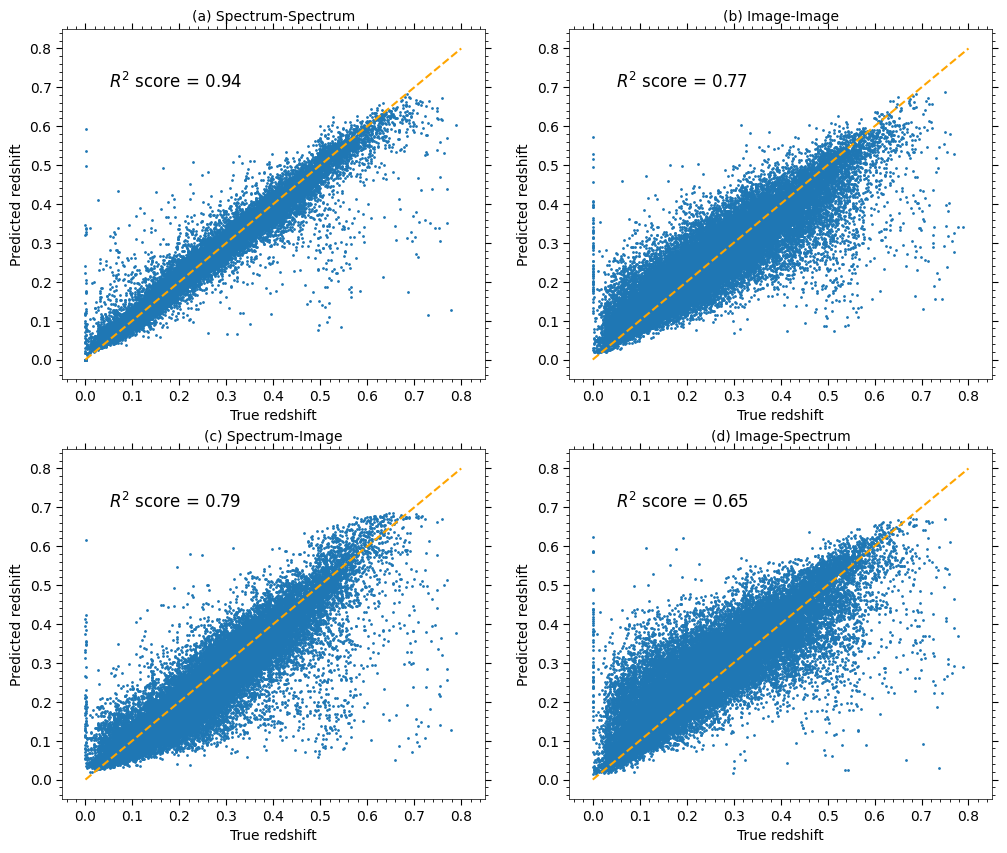
\includegraphics[width=1.2\textwidth]{figures/redshift_knn_regression}}
    \caption{In-modal and cross-modal redshift predictions using k-NN regression on the learned embeddings. The y-axis shows
    the predicted redshift (the average of the 16 closest neighbours in terms of Euclidean distance) and the x-axis shows the true redshift.
    The dashed line represents a perfect prediction, and the $R^{2}$ of the fit is shown in the top left corner.
    $S_{kNN}(\mathbf{z}_{q}^{sp}, \mathbf{z}^{im})$ indicates the cross-modal prediction where a spectrums redshift was
    predicted using its 16 closes image embedded neighbours.}
    \label{fig:rkr}
\end{figure}
